\documentclass[11pt,xcolor={dvipsnames},aspectratio=159,hyperref={pdftex,pdfpagemode=UseNone,hidelinks,pdfdisplaydoctitle=true},usepdftitle=false]{beamer}
\usepackage{presentation}[aspectratio=169]
\usepackage{math}
\usepackage{mathtools}
\usepackage{amsmath}
\usepackage{mleftright}

% Enter title of presentation PDF:
\hypersetup{pdftitle={Aggregate Shocks and Debt Management I}}
% Enter link to PDF file with figures:


\begin{document}
% Enter presentation title:
\title{Aggregate Shocks and Debt Management I}
\subtitle{Fiscal and Monetary Policy 2024}
% Enter presentation information:

% Enter presentation authors:
\author{Piotr Żoch}%
% Enter presentation location and date (optional; comment line if not needed):
\frame{\titlepage}

% Fill out content of presentation:
\begin{frame}{Plan}
    \begin{itemize}
    \item How \al{should} the government change taxes and debt in response
    to changes in purchases?
    \item For example: \al{should} it finance war spending in the same way
    as public education?
    \item This is a \al{normative} question, but to the extent real world
    governments behave according to prescriptions of models we will see
    in class, it will also be a \al{positive theory} of government debt
    and taxes.
    \end{itemize}
\end{frame}



\begin{frame}{Plan}

    \begin{itemize}
    \item We will study optimal taxation and debt policy in two environments:
    \begin{itemize}
    \item \alb{incomplete markets}: the government can buy or sell only a limited
    set of securities, often only a single risk-free security.
    \item \alr{complete markets}: the government can buy or sell claims contingent
    on all possible states of the world.
    \end{itemize}
    \item First study some reduced form models, then proceed to optimal
    taxation in a competitive equilibrium (Lucas and Stokey, 1983).
    \end{itemize}
\end{frame}
    %
    \begin{frame}
        \heading{Reduced form models}
    \end{frame}

    \begin{frame}{Incomplete Markets}
    \begin{itemize}
    \item We study the following problem based on Barro (1979):
    \begin{itemize}
    \item the government uses taxes $\tau_{t}$ to finance \emph{stochastic}
    purchases $g_{t}$;
    \item  $D\left(\tau_{t}\right)$  is the deadweight loss of taxes;
    \item the government wants to finance $g_{t}$ in a way that minimizes the
    expected value of present discounted deadweight loss of taxes: 
    \[
    \min[\bc{\tau_t}_{t=0}^\infty] \E[0] \sum_{t=0}^\infty \bs{\bp{\frac{1}{1+r}}^t D\bp{\tau_t}}
    \]
    where $1/\left(1+r\right)$ is the (gross) rate at which the government
    discounts the future.
    \end{itemize}
    \end{itemize}
    \end{frame}
    %
    \begin{frame}{Incomplete Markets}
    \begin{itemize}
    \item Assume that $g_{t}$ is governed by an $N$ state Markov chain.
    \item The state of the world is given by $s_{t}$ that follows a Markov
    chain with a transition probability matrix $P$: 
    \begin{align*}
    P_{ij} & =P\bc{s_{t+1}=\bar{s}_{j}\mid s_{t}=\bar{s}_{i}}. 
    \end{align*}
    \item Government spending $\bc{g_t}$ obeys 
    \begin{align*}
    g_{t} & =\begin{cases}
    g_{1} & \text{if}\;s_{t}=\bar{s}_{1}\\
    \vdots\\
    g_{N} & \text{if}\;s_{t}=\bar{s}_{N}.
    \end{cases}
    \end{align*}
    \end{itemize}
    \end{frame}
    %
    
    
    \begin{frame}{Incomplete Markets}
    \begin{itemize}
    \item The government can issue only \alg{one period, non-state contingent} debt (\alb{incomplete markets}) at the price $1/\left(1+r\right)$,
    equal to the discount rate. 
    \item Government problem:
    \begin{align*}
     &  \min[\bc{\tau_t}_{t=0}^\infty] \E[0] \sum_{t=0}^\infty \bs{\bp{\frac{1}{1+r}}^t D\bp{\tau_t}}\\
    \text{s.t.}\quad & g_{t}+b_{t}=\frac{1}{1+r}b_{t+1}+\tau_{t}
    \end{align*}
    and, in addition, we assume 
    \[
        \E[0] \bs{\bp{\frac{1}{1+r}}^t b^2_t} \le \infty .
    \]
    \end{itemize}
    \end{frame}
    %
    \begin{frame}{Digression on Bellman equations}
    \begin{itemize}
    \item To solve the above problem write it in a \emph{recursive} form: 
    \begin{align*}
    V\bp{b,g} & =\min[\tau] D\bp{\tau}+\frac{1}{1+r}\E\bs{V\bp{b',g'} \mid g }\\
    \text{s.t.}\quad & g+b=\frac{1}{1+r}b'+\tau
    \end{align*}
    where $x$ denotes current variables $\bp{x_{t}}$ and $x'$ denotes
    variables in the next period $\bp{x_{t+1}}$. 
    \item It looks like a two period problem (instead of infinite horizon)
    -- the ``only'' issue is that we do not know $V\bp{b,g}$
    (and it appears on the right hand side). 
    \item More on that in, for example, my Quantitative Economics course. 
    \end{itemize}
    \end{frame}
    %
    \begin{frame}{Digression on Bellman equations}
    \begin{itemize}
    \item Write
    \begin{align*}
        V\bp{b,g} & =\min[\tau] D\bp{\tau}+\frac{1}{1+r}\E\bs{V\bp{\bp{1+r}\bp{g+b-\tau},g'} \mid g }
    \end{align*}
    and differentiate with respect to $\tau$ to get the \alg{first order condition}:
    \[
    D'\bp{\tau}=\E\bs{\pd{V\bp{b',g'}}{b'} \mathrel{\Big|} g}   \]
    \item How to get $V'\bp{b',g'}\coloneqq \pdx{V\bp{b',g'}}{b'}?$
    \end{itemize}
    \end{frame}
    %
    \begin{frame}{Digression on Bellman equations}
    \begin{itemize}
    \item Write
    \begin{align*}
    V\bp{b,g} & = D\bp{g+b-\frac{1}{1+r}b'}+\frac{1}{1+r}\E\bs{V\bp{b',g'}\mid g}
    \end{align*}
    (note: there is no $\min_{\tau}$) and differentiate with respect to $b$: 
    \begin{align*}
    V'\bp{b,g} & =D'\bp{\tau}.
    \end{align*}
    This is the \alg{ envelope condition} and it implies
    \begin{align*}
    V'\bp{b',g'} & =D'\bp{\tau'}.
    \end{align*}
    \item \al{Important:} do not write $b'=b'\bp{b,g}$ or anything like
    that, these terms drop out anyway (why?).
    \end{itemize}
    \end{frame}
    %
    \begin{frame}{Digression on Bellman equations}
    \begin{itemize}
    \item The \alg{first order condition} 
    \[
        D'\bp{\tau}=\E\bs{\pd{V\bp{b',g'}}{b'} \mathrel{\Big|} g}  
    \]
    together with the \alg{envelope condition}
    \begin{align*}
        V'\bp{b',g'}  =D'\bp{\tau'}
    \end{align*}
    give us the \alg{Euler equation} 
    \begin{align*}
        D'\bp{\tau_t}  =\E[t]\bs{D'\bp{\tau_{t+1}}}
    \end{align*}
    \end{itemize}
    \end{frame}
    %
    \begin{frame}{Incomplete Markets}
    
    \begin{itemize}
    \item Solution to the government's problem is characterized by
    \[ D'\bp{\tau} =\E[t]\bs{D'\bp{\tau'}} .\]       
    \vspace{-0.76cm} 

    \item \al{Tax smoothing:} spread out distortionary effects of taxes across time.
    \item Marginal distortion of taxes today should be equal to the expected marginal distortion of taxes tomorrow.
        \end{itemize}
    
    \end{frame}


    \begin{frame}{Incomplete Markets}
        \begin{itemize}
        \item  There are two special cases we will consider in more detail:
        \begin{itemize}
            \item Special case 1 - no uncertainty (Barro, 1979):    
                 $$\tau_{t}=\tau_{t+1}$$
            \item Special case 2 - quadratic deadweight loss ($D\bp{\tau_{t}}=a\tau_{t}^{2}+\gamma):$
                $$\tau_{t}=\E[t]\bs{\tau_{t+1}}$$
        \end{itemize}
        \end{itemize}
        
        \end{frame}

    \begin{frame}{Special case 1: perfect foresight}
        \begin{itemize} 
            \item With no uncertainty about future $g_t$ (\alg{perfect foresight}), taxes are constant.
            \item $\tau$ (a single value) is chosen to satisfy the budget constraint: \[ \tau = \frac{r}{1+r} \bs{\sum_{t=0}^{\infty}\bp{1+r}^t g_t + b_0} \]
            \item Debt absorbs all fluctuations in government spending: 
            \[ b_{t+1} - b_{t} = r \bp{b_t - b_0} +  \bp{1+r}g_t - r \sum_{s=0}^{\infty}\bp{1+r}^s g_s. \]
        \end{itemize}
            
    
    \end{frame}
    
    \begin{frame}{Special case 1: perfect foresight}
        \begin{itemize} 
            \item If $g_t=g$ is constant, then \vspace{-2pt}
            \[ \tau = g + \frac{r}{1+r}b_0, \quad b_t = b_0; \] debt remains constant at its initial level. 
            \item If $g_0 = g + \epsilon$ and $g_t = g$ for all $t\geq1$ then  \vspace{-2pt}\[\tau=g+\frac{r}{1+r}\bp{\epsilon+b_0}, \quad b_t = b_0 + \epsilon;\] debt increases by $\epsilon$ and stays elevated forever.
        \item The level of debt $b_t$ is \al{irrelevant}. What matters for debt is \al{transitory} fluctuations in $g_t$, not the average level of $g_t$.
        \item Intuition valid also with trend growth of GDP and government spending (see Barro's paper). 
            \end{itemize}
            
    
    \end{frame}


    \begin{frame}{Special case 2 - quadratic deadweight loss}
    
    \begin{itemize}
    \item What does the condition \[\tau_{t}=\E[t]\bs{\tau_{t+1}}\] tell
    us about the optimal tax policy? 
    \item $\tau_{t}$ is a \alg{random walk}: 
     \begin{align*}
    \tau_{t+1}-\tau_{t} & =\tau_{t+1}-\E[t]\bs{\tau_{t+1}}\\
     & =\tau_{t+1}-\bp{\tau_{t+1}-\epsilon_{t+1}}\\
     & =\epsilon_{t+1}
    \end{align*}
    where $\epsilon_{t+1}$ is white noise.
    \end{itemize}
    \end{frame}
    %

    
    \begin{frame}{Special case 2 - quadratic deadweight loss}
    
    \begin{itemize}
    \item Taxes tomorrow expected to be the same as today, $\tau_t$ moves \al{only} because of changes in expected future $g_t$.
    \item Whenever new information is revealed, taxes immediately jump to a new level.
    \item To see this, use the budget constraint together with $\E[t]\bs{\tau_{t+1}} = \tau_t$ to get 
    \[ \tau_{t}=\frac{r}{1+r}b_{t}+\frac{r}{1+r}\sum_{s=0}^{\infty}\bp{\frac{1}{1+r}}^{s}\E[t]\bs{g_{t+s}}. \]
    so \[ \tau_t - \E[t-1]\bs{\tau_t} =\frac{r}{1+r}\sum_{s=0}^{\infty}\bp{\frac{1}{1+r}}^{s}\bp{\E[t]\bs{g_{t+s}}-\E[t-1]\bs{g_{t+s}}} \]
    \end{itemize}
    \end{frame}
    %
    \begin{frame}{Special case 2 - quadratic deadweight loss}
    
    \begin{itemize}
    \item The size of the jump in $\tau_t$ depends on the size of the change in expected future $g_t$:
    \begin{itemize} 
        \item If there is a permanent shift in $g_t$, $\E[t]\bs{g_{t+s}}-\E[t-1]\bs{g_{t+s}}=\epsilon$ for all $s$, taxes change by exactly the same amount $\epsilon$.
        \item If the change is temporary, $\E[t]\bs{g_{t+s}}-\E[t-1]\bs{g_{t+s}}=\epsilon$ only for $s=0$, taxes change by $\epsilon r \slash \bp{1+r}$.
    \end{itemize}
    \item Remaining needed resources raised through debt issuance:
    \begin{itemize}
        \item Debt remains constant for a permanent change in $g_t$.
        \item Debt changes by $\epsilon \slash \bp{1+r}$ for a temporary change in $g_t$.
    \end{itemize}

    \item \alg{Implication:} finance education by taxes, finance war by debt.
    \end{itemize}
    \end{frame}

    \begin{frame}{Special case 2 - quadratic deadweight loss}
    
        \begin{itemize}
        \item Debt also inherits the random walk property of taxes: \[\E[t]\bs{b_{t+1}}=b_t\]
        \item There is \al{nothing} that acts as a force that would push debt to a particular level:
        \begin{itemize}
            \item No debt target;
            \item No "raise taxes if debt is too high" rule;
            \item Debt is a random walk, so its variance goes to infinity unless all shocks to $g_t$ are fully permanent.
        \end{itemize}
        \end{itemize}
        \end{frame}
        %
    
        \begin{frame}{Complete Markets}
        \begin{itemize}
        \item This is a simplified version Lucas and Stokey (1983), we will see the full version later. 
        \item In the \alr{complete markets} case, the government can issue \alb{state-contingent} securities.
        \item This means that the government can issue a security that pays $1$ unit of consumption in state $s$ in the next period, and it can do it for all possible states.
        \item We call such a security an \alg{Arrow security}.
        \item Let $s_t$ denote the state in period $t$ and $s^t\coloneqq\bp{s_0,s_1,\cdots,s_t}$ denote the history of states up to period $t$.
        \item Let $q\bp{s^{t+1}\mid s^t}$ denote the period $t$ price of a security that pays $1$ unit of goods for a particular history $s^{t+1}$ in period $t+1$ (and zero in other states).
        \end{itemize}
        \end{frame}

        \begin{frame}{Complete Markets}
            \begin{itemize}
            \item To facilitate comparison with the \alb{incomplete markets} case we will assume 
            \begin{align*}
                q\bp{s^{t+1}\mid s^t} = \frac{1}{1+r} \pi\bp{s^{t+1}\mid s^t} 
            \end{align*}
            where $\pi\bp{s^{t+1}\mid s^t}$ is the conditional probability of history $s^{t+1}$ given history $s^t$.
            \item The above assumption implies: 
            \begin{align*}
                \sum_{s^{t+1} \geq  s^t} q\bp{s^{t+1}\mid s^t} = \frac{1}{1+r},
            \end{align*}
            the price of a portfolio that pays one unit of goods for sure is equal to $\bp{1+r}^{-1}$.
            \end{itemize}
            \end{frame}

        \begin{frame}{Complete Markets}
            \begin{itemize}
            \item The problem of the government is now 
            \begin{align*}  
            &\min[\bc{\tau}_{t=0}^\infty] \sum_{t=0}^\infty \sum_{s^t} \pi \bp{s^t} \bp{\frac{1}{1+r}}^t D\bp{\tau \bp{s^t}}\\
            \text{s.t.} \quad \forall s^t \quad & g\bp{s^t} + b \bp{s^{t}}=\tau\bp{s^t} + \sum_{s^{t+1} \geq  s^t} q\bp{s^{t+1}\mid s^t} b \bp{s^{t+1}}  \\
            & b \bp{s_0}  = b_0 
            \end{align*}
            where $\pi\bp{s^t}$ is the probability of history $s^t$, and $b\bp{s^t}$ is the quantitity of (negative) Arrow securities that pay in history $s^t$.
              \end{itemize}
            \end{frame}


        \begin{frame}{Complete Markets}
            \begin{itemize}
            \item We can write a Lagrangian:
            \begin{align*}  
            \sum_{t=0}^\infty \sum_{s^t} \pi \bp{s^t} \bp{\frac{1}{1+r}}^t D\bp{\tau \bp{s^t}}\\
            + \sum_{t=0}^\infty \sum_{s^t} \lambda \bp{s^t}\bs{g\bp{s^t} + b \bp{s^{t}}-\tau\bp{s^t} - \sum_{s^{t+1} \geq  s^t} q\bp{s^{t+1}\mid s^t} b \bp{s^{t+1} } }
            \end{align*}
            \end{itemize}
            \end{frame}

        \begin{frame}{Complete Markets}
            \begin{itemize}
            \item First order condition with respect to $\tau \bp{s^t}$:
            \begin{align*}  
                \pi \bp{s^t} \bp{\frac{1}{1+r}}^t D' \bp{\tau \bp{s^t}} =  \lambda\bp{s^t}
            \end{align*}
            \item First order condition with respect to  $b \bp{s^{t+1}}$:
            \begin{align*}
                q\bp{s^{t+1}\mid s^t} \lambda\bp{s^t} = \lambda\bp{s^{t+1}} 
            \end{align*}
            \end{itemize}
            \end{frame}

            \begin{frame}{Complete Markets}
                \begin{itemize}
                \item Given the assumption              
                \begin{align*}
                    q\bp{s^{t+1}\mid s^t} = \frac{1}{1+r} \pi\bp{s^{t+1}\mid s^t} 
                \end{align*}
                we have 
                \begin{align*}  
                    \frac{1}{1+r} \pi\bp{s^{t+1}\mid s^t}  \lambda\bp{s^t} = \lambda\bp{s^{t+1}} 
                \end{align*}
                so 
                \begin{align*}
                    \frac{1}{1+r} \pi\bp{s^{t+1}\mid s^t} \pi \bp{s^t} \bp{\frac{1}{1+r}}^t D' \bp{\tau \bp{s^t}} \\ =   \pi \bp{s^{t+1}} \bp{\frac{1}{1+r}}^{t+1} D' \bp{\tau \bp{s^{t+1}}}
                \end{align*}
                \end{itemize}
                \end{frame}

    \begin{frame}{Complete Markets}
        \begin{itemize}
        \item It simplifies to              
        \begin{align*}
                D' \bp{\tau \bp{s^t}} =   D' \bp{\tau \bp{s^{t+1}}}
        \end{align*}
        i.e.
        \begin{align*}  
            \tau \bp{s^t} =   \tau \bp{s^{t+1}}.
        \end{align*}
        \item This is the \al{key result}: \alg{perfect smoothing of taxes across states}.
        \item The result holds \alr{regardless} of the form of $D\bp{\tau}$ or the nature of risk.
        \item Compare it with incomplete markets case: it was true only with perfect foresight.
        \end{itemize}
        \end{frame}

        \begin{frame}{Complete Markets}
            \begin{itemize}
            \item What about debt?          
            \item Guess that $b\bp{s^{t+1}}$ depends only on the future state $s_{t+1}$, and not on the history $s^t$.
            \item Intuitively: the government cares only about the future state, not about the history (why?).
            \item Use this guess together with $\tau \bp{s^t} =   \tau$ and the initial condition $b\bp{s_0} = b_0$ to solve for $\tau$ and optimal debt policy.
            \item This also verifies the guess.
        \end{itemize}
            \end{frame}

        \begin{frame}{Complete Markets}
            \begin{itemize}
            \item Since $b\bp{s^{t+1}}=b\bp{s_{t+1}}$, debt neither accumulates, nor decumulates, nor drifts -- it switches between different levels.
            \end{itemize}
            \end{frame}

            \begin{frame}{Comparison}
                \begin{itemize}
                \item \alb{Incomplete}: taxes drift over time as a random walk; the level of taxes at time $t$ depends on the level of debt that the government brings into the period as well as the expected discounted present value of government purchases.
                \item \alr{Complete}: taxes are constant, regardless of the state of the world; the level of taxes at time $t$ is independent of the level of debt that the government brings into the period.
                \end{itemize}
            \end{frame}

            \begin{frame}{Comparison}
                \begin{itemize}
                \item \alb{Incomplete}: debt drifts upward over time in response to large purchases and drifts downward over time in response to low purchases.
                \item \alr{Complete}: debt osciallates between several levelsl; this is akin to the government purchasing insurance that protects against the need to raise taxes too high or issue too much debt in the high government expenditure event.
                \end{itemize}
            \end{frame}

            \begin{frame}{Numerical example}
                \begin{itemize}
                \item Let $\bp{1+r} ^{-1} = 0.96$ and there are two levels of government purchases: $g_1 = 1$ and $g_2 = 2$ with
                with transition probabilities $P_{12} = 0.2$ and $P_{21}= 0.4$.
                \item The initial condition is $b_0 = 0$, and we start with $g_1$.
                \end{itemize} 
            \end{frame}

            \begin{frame}{Numerical example}
                \begin{figure}
                    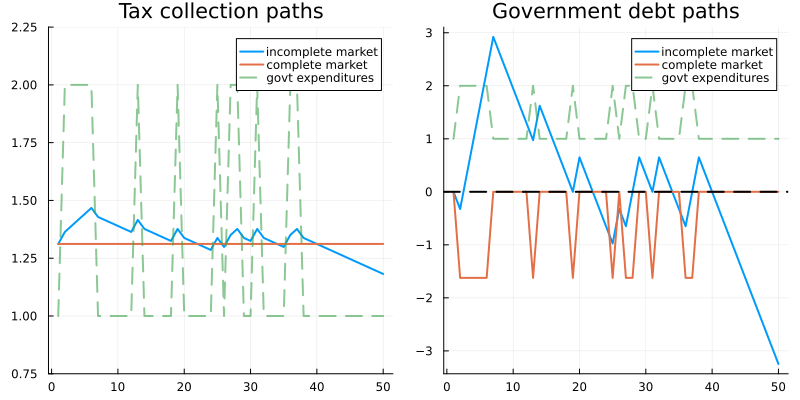
\includegraphics[width=0.9\textwidth]{plot.png}
                    \caption{Tax and debt policy in complete and incomplete markets. Computed using QuantEcon Julia package.} 
                \end{figure}

            \end{frame}

            \begin{frame}
                \heading{Lucas and Stokey (1983)}
            \end{frame}
        
            \begin{frame}{Setup}
            \begin{itemize}
            \item We study the following problem based on Lucas and Stokey (1983):
            \begin{itemize}
            \item the representative household has preferences over consumption and labor (leisure);
            \item production technology is linear in labor, there is no capital;
            \item the government uses \al{distortionary} tax rate $\tau_{t}$ on \al{labor income} to finance \emph{stochastic}
            purchases $g_{t}$ (we assume $g_{t}$ is a Markov process);
            \item the households and the government can trade a full set of \alg{Arrow securities} (state-contingent claims).
            \item the government wants to finance $g_{t}$ in a way that maximizes the welfare of the representative household.
            \end{itemize}
            \item General equilibrium.
            \end{itemize}
            \end{frame}
        
        
            %
            \begin{frame}{Setup}
            \begin{itemize}
            \item Price of securities no longer exogenous.
            \item The government's cares about welfare of the representative household.
            \item Think of the problem in two steps:
            \begin{enumerate} 
                \item for \al{given} government policies there exists some \alg{competitive equilibrium};
                \item the government picks policies that result in the "best" equilibrium.
            \end{enumerate}
            \item Key difference: policies not only have to satisfy the government's budget constraint, but also household's optimality conditions.
            \item \alb{Primal approach}: we will look directly for allocations that maximize welfare and then think of policies that implement that.
            \end{itemize}
            \end{frame}
            %
            \begin{frame}{Competitive equilibrium}
                \begin{beamerboxesrounded}[upper=block head,lower=block body,shadow=false]{\textbf{Competitive equilibrium}}
                    A competitive equilibrium given government policies $\tau\bp{s^t}$ and $g\bp{s^t}$ is a set of allocations $\bp{c\bp{s^t},\ell\bp{s^t},a\bp{s^{t+1}}}$ and prices $\bp{q\bp{s^{t+1} \mid s^t },w\bp{s^t}}$ such that: 
                    \begin{enumerate}
                        \item Given prices, allocations solve the household problem;
                        \item Given prices, allocations solve the firm problem;
                        \item The government budget constraint is satisfied is each state;
                        \item All markets clear in each state.
                    \end{enumerate}
                \end{beamerboxesrounded}
        
                \begin{itemize}
                    \item Note: this is not a proper definition of a competitive equilibrium, but it will do for our purposes.
                \end{itemize}
                \end{frame}
            
            \begin{frame}{Household problem}
            \begin{itemize}
            \item Household chooses consumption, labor supply and portfolio of Arrow securities to maximize expected utility:
            \item Household problem:
            \begin{align*}  
                &\max \E_0 \sum_{t=0}^\infty  \beta^t u\bp{c \bp{s^t},\ell\bp{s^t}}\\
                \text{s.t.} \quad \forall s^t \quad & c\bp{s^t}  + \sum_{s^{t+1} \geq  s^t} q\bp{s^{t+1}\mid s^t} a \bp{s^{t+1}} \\ &=\bp{1 - \tau\bp{s^t} }w \bp{s^t} \ell\bp{s^t} + a \bp{s^{t}}  \\
                & a \bp{s^0}  = a_0 
                \end{align*}
                where $u\bp{\cdot}$ is the utility function, $c\bp{\cdot}$ consumption and $\ell \bp{\cdot}$ labor.
                  \end{itemize}
            \end{frame}
        
        
            \begin{frame}{Household problem}
            \begin{itemize}
            \item The sequence of household budget constraints can be written as a single constraint
            \begin{align*}  
            \sum_{t=0}^\infty \sum_{s^t}  q\bp{s^t} c\bp{s^t}  =
            \sum_{t=0}^\infty \sum_{s^t}  q\bp{s^t} \bp{1 - \tau\bp{s^t} }w \bp{s^t} \ell\bp{s^t} +q\bp{s^0} a_0 
            \end{align*}
            where $q\bp{s^t}$ is now the time-0 price of one unit of goods in state $s^t$.
            \item Why? \al{Complete markets} are \alg{equivalent} with Arrow securities and time-0 trading.
                \end{itemize}
            \end{frame}
        
            \begin{frame}{Household problem}
            \begin{itemize}
            \item Household problem:
            \begin{align*}  
                & \max \sum_{t=0}^\infty \sum_{s^t}  \beta^t \pi\bp{s^t} u\bp{c \bp{s^t},\ell\bp{s^t}}\\
                \text{s.t.} & \sum_{t=0}^\infty \sum_{s^t}  q\bp{s^t} c\bp{s^t}  =
                \sum_{t=0}^\infty \sum_{s^t}  q\bp{s^t} \bp{1 - \tau\bp{s^t} }w \bp{s^t} \ell\bp{s^t} \\ &  + q\bp{s^0}a_0 
                \end{align*}
                \item This is nice because there is only \al{one} constraint. 
                    \end{itemize}
            \end{frame}
        
        
            %
            \begin{frame}{First order conditions}
            \begin{itemize}
            \item Write down the Lagrangian and differentiate with respect to $c\bp{s^t}$ and $\ell\bp{s^t}$ to get the first order conditions:
            \begin{align*}
            \bs{c\bp{s^t}:} \;\beta^t \pi\bp{s^t} u_c \bp{c \bp{s^t},\ell\bp{s^t}} & =\lambda q\bp{s^t}\\
            \bs{\ell\bp{s^t}:} \;\beta^t \pi\bp{s^t} u_{\ell} \bp{c \bp{s^t},\ell\bp{s^t}} & =-\lambda q\bp{s^t}\bp{1 - \tau\bp{s^t} }w \bp{s^t}
            \end{align*}
            \item Note: the Lagrange multiplier $\lambda$ is \alg{the same} for all states $s^t$.
            \item To simplify notation 
            \begin{align*}
                \bs{c\bp{s^t}:} \;\beta^t \pi\bp{s^t} u_c \bp{s^t} & =\lambda q\bp{s^t}\\
                \bs{\ell\bp{s^t}:} \;\beta^t \pi\bp{s^t} u_{\ell} \bp{s^t} & =-\lambda q\bp{s^t}\bp{1 - \tau\bp{s^t} }w \bp{s^t}
                \end{align*}
            \end{itemize}
            \end{frame}
        
        \begin{frame}{Implementability constraint}
                \begin{itemize}
                    \item The first order conditions:
                \begin{align*}
                    \bs{c\bp{s^t}:} \;\beta^t \pi\bp{s^t} u_c \bp{s^t} & =\lambda q\bp{s^t}\\
                    \bs{\ell\bp{s^t}:} \;\beta^t \pi\bp{s^t} u_{\ell} \bp{s^t} & =-\lambda q\bp{s^t}\bp{1 - \tau\bp{s^t} }w \bp{s^t}
                \end{align*}
                    together with the budget constraint
                \begin{align*}
                    \sum_{t=0}^\infty \sum_{s^t}  q\bp{s^t} c\bp{s^t}  =
                    \sum_{t=0}^\infty \sum_{s^t}  q\bp{s^t} \bp{1 - \tau\bp{s^t} }w \bp{s^t} \ell\bp{s^t}  + q\bp{s^0}a_0   
                \end{align*}
                allow us to write the \alb{implementability constraint}:
                 \begin{align*}  
                    \sum_{t=0}^\infty \sum_{s^t} \beta^t \pi\bp{s^t} \bs{  u_c \bp{s^t} c\bp{s^t}  + u_{\ell} \bp{s^t} \ell\bp{s^t}}  = u_c \bp{s^0} a_0
                \end{align*}
                \end{itemize}
            \end{frame}
            \begin{frame}{Implementability constraint}
                \begin{itemize}
                    \item The \alb{implementability constraint}
                    \begin{align*}  
                        \sum_{t=0}^\infty \sum_{s^t} \beta^t  \pi\bp{s^t} \bs{  u_c \bp{s^t} c\bp{s^t}  + u_{\ell} \bp{s^t} \ell\bp{s^t}}  = u_c \bp{s^0} a_0
                    \end{align*}
                summarizes household optimality conditions and the budget constraint.
                \item The government can only choose allocations that satisfy this constraint.
                \item Captures the notion that the government's choices result in some \al{optimal} (given these choices) household behavior.
                \end{itemize}
            \end{frame}
            
            \begin{frame}{Firm problem}
                \begin{itemize}
                    \item Output in this economy is produced by a representative price-taking firm.
                    \item Linear production function that uses labor as an input.
                    \item Firm problem is almost trivial -- it chooses labor to maximize profits:
                    $$\max_{\ell\bp{s^t}}\; A\ell\bp{s^t} - w\bp{s^t} \ell \bp{s^t}.$$
                    \item In a competitive equilibrium we must have
                    $$ w\bp{s^t} = A.$$
                \end{itemize}
            \end{frame}
            \begin{frame}{Government budget constraint}
                \begin{itemize}
                    \item The \alb{implementability constraint} is the household budget constraint (+ optimality conditions)
                    \item The government should also be constrained by its budget constraint.
                    \item We can ignore it and focus \al{directly} on the \al{resource constraint} of the economy: 
                    $$ A \ell\bp{s^t} = g\bp{s^t} + c\bp{s^t}$$
                    where $A \ell\bp{s^t}$ is the linear production technology.
                    \item Why? \al{Walras' law} -- the government budget constraint is redundant.
                \end{itemize}
            \end{frame}
            
        
        
            \begin{frame}{Government problem}
            \begin{itemize}
            \item The government chooses \alg{allocations} $c\bp{s^t},\ell\bp{s^t}$ to maximize the household's utility 
            \begin{align*}
                \sum_{t=0}^\infty \sum_{s^t}  \beta^t \pi\bp{s^t} u\bp{c \bp{s^t},\ell\bp{s^t}}
            \end{align*}
            subject to the \alb{implementability constraint}:
            \begin{align*}  
                \sum_{t=0}^\infty \sum_{s^t}  \beta^t \pi\bp{s^t} \bs{  u_c \bp{s^t} c\bp{s^t}  + u_{\ell} \bp{s^t} \ell\bp{s^t}}  = u_c \bp{s^0} a_0
            \end{align*}
            and \al{resource constraints}: 
            \begin{align*}
            \forall s^t \quad   A \ell\bp{s^t} = g\bp{s^t} + c\bp{s^t}
            \end{align*}
            \end{itemize}
            \end{frame}
            %
        \begin{frame}{Government problem}
            \begin{itemize}
            \item \alg{Full commitment}: the government announces its state-contingent plans at time 0 and cannot change them later.
            \item Everyone else trusts the government and knows it will stick to its plans.
            \end{itemize}   
            \end{frame}
        
            \begin{frame}{Optimality conditions}
            \begin{itemize}
            \item The \alg{first order conditions} for $s^t > s^0$ (we will return to $s^0$ later):
            \begin{align*}
              u_c\bp{s^t} + \eta \bs{ u_{cc} \bp{s^t} c\bp{s^t} + u_c \bp{s^t} + u_{c\ell} \bp{s^t} \ell\bp{s^t} }  & =  \mu \bp{s^t} \\
              u_\ell\bp{s^t} +\eta \bs{ u_{c\ell} \bp{s^t} c\bp{s^t} + u_\ell \bp{s^t} + u_{\ell\ell} \bp{s^t} \ell\bp{s^t} }  & =  - \mu \bp{s^t} A
            \end{align*}
            where $\eta$ is the Lagrange multiplier on the \alb{implementability constraint} and $\mu\bp{s^t}$ is the Lagrange multiplier on the \al{resource constraint}.
            \item There is also a resource constraint for each state: 
            \begin{align*}
                A \ell\bp{s^t} = g\bp{s^t} + c\bp{s^t}
            \end{align*}
            \item This gives us, for each state, three equations in three unknowns: $c\bp{s^t},\ell\bp{s^t},\mu\bp{s^t}$.
            \end{itemize}
            \end{frame}
            %
            \begin{frame}{Optimality conditions}
                \begin{itemize}
                \item We also have a fourth unknown: $\eta$ and one more equation: the \alb{implementability constraint}.
                \item Key: $\eta$ is the \al{only} link between different states.
                \item Once we know it, $c\bp{s^t},\ell\bp{s^t},\mu\bp{s^t}$ are determined for each $s^t$ from 2 first order conditions and the resource constraint.
                \item For two different states with the same $g\bp{s^t}$, the solution must be the same!
            \end{itemize}
                \end{frame}
        
            \begin{frame}{Implications}
                \begin{itemize}
                \item What are the implications for taxes?
                \item From household first order condition we have 
                \begin{align*}
                    \bp{1-\tau\bp{s^t}} w\bp{s^t} = - \frac{u_\ell\bp{s^t}}{u_c\bp{s^t}}
                \end{align*}
                and linear production technology implies $w\bp{s^t} = A$ so
                \begin{align*}
                    1-\tau\bp{s^t}  = - \frac{u_\ell\bp{c \bp{s^t},\ell\bp{s^t}}}{u_c\bp{c \bp{s^t},\ell\bp{s^t}}} \frac{1}{A}.
                \end{align*}
                \item We have solved for $c \bp{s^t},\ell\bp{s^t}$, we can get $\tau\bp{s^t}$!
                \end{itemize}
            \end{frame}
                    
            \begin{frame}{Implications}
                \begin{itemize}
                \item Since for two different states with the same $g\bp{s^t}$ consumption and labor are the same -- taxes must be the same!
                \item \alg{Conclusion:} very different from Barro (1979) -- no history dependence.
                \item If government purchases are i.i.d., taxes are i.i.d. as well.
                \item Contrast with the \alb{incomplete markets case}: taxes were a random walk.
                \item Contrast with the \alr{reduced form complete markets case}: taxes were constant.
                \end{itemize}
            \end{frame}
        
            \begin{frame}{Implications}
                \begin{itemize}
                \item Why is the result different from the reduced form complete markets case?
                \item No full tax smoothing (unless with particular household preferences), because of a different objective.
                \item When $g_t$ is high, the government could want to \al{increase} labor supply to finance it without a large drop in consumption.
                \end{itemize}
            \end{frame}
        
        
            \begin{frame}{Example}
                \begin{itemize}
                \item Let $u\bp{\cdot} = \frac{c^{1-\gamma}}{1-\gamma} - \psi \ell $.
                \item Then $u_c = c^{-\gamma}$, $u_{cc} = -\gamma c^{-\gamma-1}$, $u_{\ell} = -\psi$, $u_{\ell\ell} = 0$, $u_{c\ell} = 0$.
                \item The first order conditions 
              \begin{align*}
                    u_c\bp{s^t}  + \eta \bs{ u_{cc} \bp{s^t} c\bp{s^t} + u_c \bp{s^t} + u_{c\ell} \bp{s^t} \ell\bp{s^t} } & =  \mu \bp{s^t} \\
                    u_\ell\bp{s^t}  + \eta \bs{ u_{c\ell} \bp{s^t} c\bp{s^t} + u_\ell \bp{s^t} + u_{\ell\ell} \bp{s^t} \ell\bp{s^t} } & =  - \mu \bp{s^t} A
                  \end{align*}
                  are
                  \begin{align*}
                    \bs{1+\eta\bp{1-\gamma}} c\bp{s^t}^{-\gamma} & =  \mu \bp{s^t} \\
                    \bs{1+\eta}\psi & =   \mu \bp{s^t} A
                  \end{align*}
                    
                \end{itemize}
            \end{frame}
        
            \begin{frame}{Example}
                \begin{itemize}
                \item For each state $s^t>s^0$ we have:
                \begin{align*}
                    \frac{1+\eta}{\bs{1+\eta\bp{1-\gamma}}A}\psi & =   c\bp{s^t}^{-\gamma}
                \end{align*}
                so consumption is constant.
                \item Taxes satisfy  
                \begin{align*}
                1-\tau\bp{s^t}  =  \frac{\psi}{c\bp{s^t}^{-\gamma}} \frac{1}{A}:
                \end{align*}
                since $c\bp{s^t}$ is constant, taxes are \al{constant} as well.
                \item With these preferences households supply labor fully elastically, fluctuations in $g_t$ are absorbed by changes in production.
                \end{itemize}
            \end{frame}
            
            \begin{frame}{Lessons}
                \begin{itemize}
                \item \al{Rembember:} the above result is \al{not} general.
                \item What is general is that here allocations and taxes are \al{history independent} -- they are fully determined by the \alg{current} state.
                \item What is the optimal path of debt? Similar logic as in the reduced form case: state-contingent debt that depends only on the next period state.
                \end{itemize}
            \end{frame}   
        
            \begin{frame}{Time-0}
                \begin{itemize}
                \item We ignored one important issue: \alg{first order conditions} are different for period 0. 
                \item This is because of the $u_c\bp{s^0} a_0$ term in the \alb{implementability constraint}.
                \item First order conditions for $s^0$ are:    
                \footnotesize
                 \begin{align*}
                    u_c\bp{s^0}+ \eta \bs{ u_{cc} \bp{s^0} c\bp{s^0} + u_c \bp{s^0} + u_{c\ell} \bp{s^0} \ell\bp{s^0} - u_{cc} \bp{s^0} a_0 }  & =  \mu \bp{s^0} \\
                    u_\ell\bp{s^0}+\eta \bs{ u_{c\ell} \bp{s^0} c\bp{s^0} + u_\ell \bp{s^0} + u_{\ell\ell} \bp{s^0} \ell\bp{s^0} - u_{c\ell} \bp{s^0} a_0  }  & =  - \mu \bp{s^0} A
                  \end{align*}
                  \normalsize
                \item Time-0 allocations will be different from other periods, even with the same level of $g_t$.
            \end{itemize}
            \end{frame}   
        
            \begin{frame}{Time-0}
                \begin{itemize}
                \item The government has incentives to play with taxes in period 0 to change $q\bp{s^0}$ and thus affect the value of debt/assets.
                \begin{itemize}
                    \item For example: it could try to make debt due at time 0 worthless.
                    \item This is \alg{good}, because it allows the government to create \alg{lower} tax distortions in the future.
                \end{itemize}
               \item No similar effect in other periods, forward looking agents take it into account.
            \end{itemize}
            \end{frame}   
        
        
            \begin{frame}{Time inconsistency}
                \begin{itemize}
                \item \al{Time consistency problem}: if the government could re-optimize at future dates, period 1 would be like period 0. 
                \item Same logic applies to all other periods.
                \item But forward-looking agents would know the government is tempted to do it every period!
                \item This is actually the essence of Lucas and Stokey (1983).
                    \begin{itemize}
                                \item Is there a way to design debt portfolio (maturities etc.) to ensure the government will \al{not be tempted} to re-optimize?
                    \end{itemize}
            \end{itemize}
            \end{frame}   
\end{document}